\documentclass[tikz,border=12pt]{standalone}
% Estilo comum dos esquemas vetoriais das aulas da GA033.
\usepackage[T1]{fontenc}
\usepackage[utf8]{inputenc}
\usepackage{lmodern}
\usepackage{amsmath,amssymb}
\usetikzlibrary{arrows.meta,positioning,calc,fit,matrix,decorations.pathreplacing,backgrounds,shapes.geometric}
\definecolor{lnccblue}{HTML}{075AC0}
\definecolor{ink}{HTML}{242A31}
\definecolor{muted}{HTML}{647080}
\definecolor{lightblue}{HTML}{EFF5FC}
\definecolor{teal}{HTML}{197C83}
\definecolor{orange}{HTML}{BC6A16}
\tikzset{
  every node/.style={font=\sffamily\fontsize{15}{18}\selectfont,text=ink},
  box/.style={draw=lnccblue,line width=0.9pt,fill=lightblue,inner sep=9pt,align=center},
  flow/.style={-{Stealth[length=3mm,width=2mm]},draw=lnccblue,line width=1pt},
  point/.style={circle,draw=lnccblue,fill=white,line width=1.2pt,minimum size=3.2mm,inner sep=0pt},
  label/.style={font=\sffamily\fontsize{13}{16}\selectfont,text=muted},
  heading/.style={font=\sffamily\bfseries\fontsize{16}{19}\selectfont,text=lnccblue}
}
% Impede setas horizontais involuntariamente invertidas após editar os nós.
\newdimen\origemseta
\newdimen\destinoseta
\newcommand{\verificarsetadireita}[2]{%
  \pgfextractx{\origemseta}{\pgfpointanchor{#1}{east}}%
  \pgfextractx{\destinoseta}{\pgfpointanchor{#2}{west}}%
  \advance\origemseta by 4mm%
  \ifdim\destinoseta>\origemseta\else
    \PackageError{diagramas}{Conector sem espaco entre #1 e #2}{Afaste os nos antes de compilar.}%
  \fi
}

\begin{document}
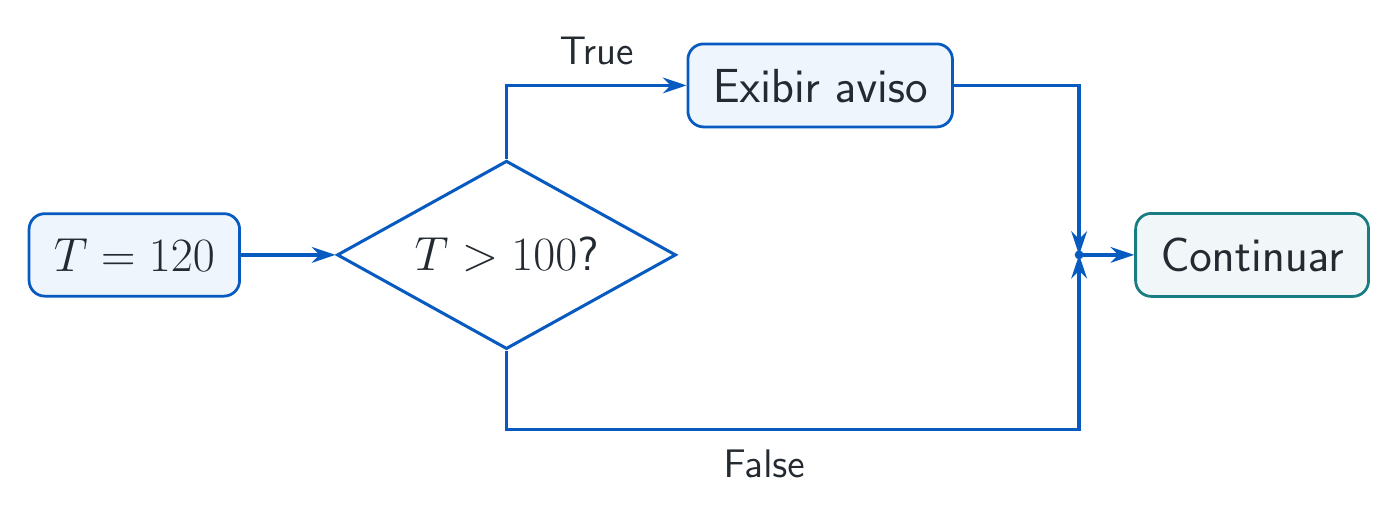
\begin{tikzpicture}[
  every node/.append style={font=\sffamily\fontsize{17}{21}\selectfont},
  etapa/.style={draw=lnccblue,fill=lightblue,rounded corners=2mm,
    line width=1pt,align=center,inner sep=9pt,minimum height=.95cm},
  seta/.style={-{Stealth[length=3mm,width=2mm]},draw=lnccblue,line width=1.2pt}
]
\node[etapa] (entrada) {$T=120$};
\node[diamond,aspect=1.8,draw=lnccblue,fill=white,line width=1.1pt,
  inner sep=6pt,right=12mm of entrada] (decisao) {$T>100$?};
\node[etapa,above right=10mm and 12mm of decisao] (aviso) {Exibir aviso};
\node[etapa,draw=teal,fill=teal!6,right=58mm of decisao] (continua) {Continuar};
\coordinate (encontro) at ($(continua.west)+(-7mm,0)$);
\coordinate (falso) at ($(decisao.south)+(0,-10mm)$);
\verificarsetadireita{entrada}{decisao}
\verificarsetadireita{aviso}{encontro}
\verificarsetadireita{encontro}{continua}
\draw[seta] (entrada.east) -- (decisao.west);
\draw[seta] (decisao.north) |- (aviso.west);
\node[above=4pt,font=\sffamily\fontsize{15}{18}\selectfont]
  at ($(decisao.north |- aviso.west)!0.5!(aviso.west)$) {True};
\draw[seta] (aviso.east) -| (encontro);
\draw[seta] (decisao.south) -- (falso) -| (encontro);
\node[below=4pt,font=\sffamily\fontsize{15}{18}\selectfont]
  at ($(falso)!0.45!(falso -| encontro)$) {False};
\fill[lnccblue] (encontro) circle[radius=1.6pt];
\draw[seta] (encontro) -- (continua.west);
\end{tikzpicture}
\end{document}
